\chapter{Literature Review}
\label{chap:lit_rev}
This chapter has two sections. One aims to review past results from literature in the field of optical character recognition. The second one presents the theoretical background of the methods used in the OCR engine. 

\section{Related Work}
\subsection{Character Recognition and Segmentation}
One of the most popular machine learning datasets is the MNIST dataset of handwritten digits\cite{lecun1998mnist}, that is used to evaluate the performance of machine learning algorithms for recognizing characters. This dataset contains 60000 examples to be used for training and 10000 to be used as a test set. All the black and white (bilevel) images in this data set were initially size normalized to fit a 20x20 bounding box, while preserving aspect ratio. The resulting images were anti-aliased, which introduced grey levels. In the end, the images were centered in 28x28 image, translating the center of mass of the pixels to the center of the 28x28 image. 

Initial results on the MNIST database, from the paper published by Y. LeCun and L. Bottou in 1998\cite{Lecun_1998}, are summarized in Table \ref{table:mnist_results}. 

\begin{table}[h]
\caption{Test error rates obtained on MNIST using various algorithms}
\label{table:mnist_results}
\begin{tabular}{ll}
\hline
Classifier                   & Test error rate \\ \hline
1-layer neural network       & 12.0 \%           \\
K-nearest-neighbors          & 5.0  \%           \\
PCA + quadratic classifier   & 3.3  \%          \\
SVM with Gaussian Kernel     & 1.4  \%           \\
2-layer neural network       & 4.7  \%           \\
3-layer neural network       & 2.45 \%           \\
Convolutional neural network & 0.95 \%           \\ \hline
\end{tabular}
\end{table}

Many improvements have been published on the MNIST dataset. Some of the more recent ones include L. Deng and D. Yu\cite{deng2011deep}, obtaining an error rate of 0.83\%, using a deep convex neural net with unsupervised pre-training. The best result obtained without using committees is D. Ciresan's deep neural network, trained on GPU devices\cite{Cire_an_2010}, that obtained 0.35\% error rate. The current state of the art was obtained by the same group, using a committee of 35 convolutional neural networks, with an error rate of 0.23\%, which beats human performance\cite{2012arXiv1202.2745C}. 

For the character segmentation problem, one approach proposed by S. Lee and D. Lee\cite{Dong_June_Lee} was based on vertical projections of the images. The projections were obtained by counting how many black pixels were in a column and then various criteria were used to determine which columns were candidates for segmentation, based on some threshold values. They obtained results ranging from 85\% to 98\% accuracy, depending on font and alphabet that was used. 

F. Kahraman and B. Kurt used a nonlinear vector quantization to perform the character segmentation\cite{kahraman2003license} with an accuracy of 94.5\% on a set of 2198 license plate characters. 

F. Vojt{\v{e}}ch and H. V{\'{a}}clav presented in \cite{Franc_2005} an approach using Hidden Markov Chains to model the problem of character segmentation in license plates. Without incorporating prior knowledge about the license plate, they got 37\% incorrect segmentations, but by using that knowledge, they managed to get it down to 3.3\%.

\subsection{OCR Engines}
Optical character recognition has long been of interest in the computer industry. In 1976, Ray Kurzweil presented in \cite{schantz1982history} an omni-font OCR engine, that together with a speech synthesiser would read texts to blind people. It came together with its own special scanner, that was required for taking the images of pages. 

R. Holley presents in a study\cite{Holley_2009} done to evaluate OCR on australian newspapers that the accuracy of various commercial software on newspapers varies from 71\% to 98\%. A similar study done by E. Klijn in \cite{klijn2008current} on Dutch newspapers reported accuracies varying between 68\% to 99\%, with this number depending mostly on the quality of the image scan and on the state of the newspaper. 

B. Janssen and E. Saund have worked on a system called Receipts2Go\cite{janssen2012receipts2go} for extracting information from small documents, including receipts. They presented two improvements to the image normalization process, but for the actual OCR part they used off-the-shelf commercial software. 

One of the most popular open-source OCR engines is Tesseract, presented in \cite{smith2007overview}. It was developed originally at HP between 1984 and 1994, where it was part of the software distributed with HP's flatbed scanners. Because of this, Tesseract doesn't perform any document layout analysis, instead it assumes that the input is a binary image with text in polygonal areas. 

The first thing Tesseract does on the input image is to find the connected components and store the outlines of the components. These outlines are nested together and they form blobs. These blobs are then filtered by a simple percentile height filter so that the drop caps and vertically touching characters are removed. The median height of the remaining blobs is used to approximate the size of the text, filtering the ones that are much smaller than it. The remaining blobs are then fit to a series of non-overlapping, parallel lines that can be sloped. After the fitting is done, the previously filtered blobs are reinserted into their lines. 

After this, the baseline for the text is calculated by fitting a quadratic spline to the most populous partition. Using a quadratic spline allows for detection of curved baselines, which often occur when scanning books. The text is then test to determine whether it has fixed pitch (all letters have the same width) or proportional text spacing. In the first case it just segments the letters using the detected pitch, while in the second case some of the spaces it detects are fuzzy, the decision to segment being left until the word recognizer has run. 

Before starting to recognize characters, Tesseract has to decide how to segment words into characters. The first step is to identify any joined characters that need to be chopped. Candidates for this are found from the concave vertices of the polygonal approximations of the outline that have another concave vertex opposite them or that are across a line segment. After this Tesseract considers joining characters that might have been broken into pieces. This done with an A* search of the segmentation graph of possible combinations of chopped blobs. 

All this is then passed into the character classifier, which has two parts: a static classifier and an adaptive one. Tesseract does a first pass with its static classifier, which extracts between 50 and 100 features per character and compares them to the prototypes it has learned during original training. Limited linguistic analysis is then done, where the linguistic module chooses the best words that fit best the given segmentation. After this, there is another pass done with the adaptive classifier, which is similar to the static classifier, but instead of using fixed prototypes, it normalizes characters by isotropic baseline and x-height, and uses the letters it has recognized with high confidence previously to retrain itself. 

Another popular open-source engine is OCRopus \cite{breuel2008ocropus}, which is newer, initially launched in 2007. It is designed to be modular, all of its components being pluggable: the layout analysis, the character recognition and the language modeling. Its main purpose is to be used for large-scale digital library applications.

The architecture of OCRopus has three components: physical layout analysis, responsible for identifying text columns, blocks and lines; text line recognition, responsible for recognizing the text from each line; and a statistical language modeling unit which corrects errors made in the previous step by incorporating domain knowledge about the language and the vocabulary of the document. 

For the layout analysis, the input image is first divided into candidate regions. These are then classified using logistic regression into different categories, such as text, image, drawing and other. Then the columns are identified using the maximal whitespace rectangle algorithm. Then lines are matched in the bounding boxes found in each column and then their reading order is determined. 

To recognize text lines, OCRopus can use either Tesseract or its own, multilayer perceptron (MLP) based recognizer. The MLP one first does an oversegmentation of the input which results in a hypothesis graph. Then for each character it extracts features, such as gradients, singular points, the presence of holes and other geometric information which are then used to obtain the posterior probability for each character class. 

The language modeling part of OCRopus is done using dictionaries, characater-level and word-level n-grams and stochastic grammars. It represents the statistical language models as weighted finite state transducers, which are a generalization of hidden Markov models and finite state transducers. These are used to resolve ambiguous or missing characters from words, to their most probable value. 

\section{Theoretical Background}

\subsection{Random forests}

Random forests have been introduced by Leo Breiman and Adele Cutler\cite{breiman2001random} as an ensemble of decision trees. When using only one decision tree to make a classification, one often runs into problems with high variance or high bias. Random forests present a mechanism to avoid these problems to make more accurate models, that generalize better. 

According to their definition given by Leo in \cite{breiman2001random}, ``a random forest is a classifier consisting of a collection of tree-structured classifiers $ \{h(x, \theta_k), k=1, ... \} $, where the $ \{ \theta_k \} $ are independent identically distributed random vectors and each tree casts a unit vote for the most popular class at input $ x $''.


When training the random forest, for each tree, n samples are taken with replacement from the training data (a bootstrap sample) and the tree is trained on these, using a slightly modified procedure. When splitting in a node, instead of choosing the best split across all features, as is done in the classical decision tree approach, here the best split is chosen from a random subset of the m features. This is done to avoid correlations between trees: otherwise good features would always get picked in all trees, so they would be correlated. As m is smaller, the correlation between the trees is smaller, but the strength of each tree (how well it can predict on its own) also goes down, so a balance must be found between these extremes. 

Random forests are a popular algorithm in many machine learning competitions, because they are fast, they don't have many parameters to tune, yet still produce good predictions. Among their weaknesses is the fact that they can easily overfit a noisy dataset. 

\subsection{Support Vector Machines}

Support vector machines\cite{Cortes_1995} are discriminative classifiers formally defined by high-dimensional hyperplanes, which are used to distinguish between the classes to which data points belong. The hyperplane defined by an SVM maximizes the margin to the data points used in training, hoping that this leads to a better generalization of the classifier. 

\begin{figure}[h]
\begin{center}
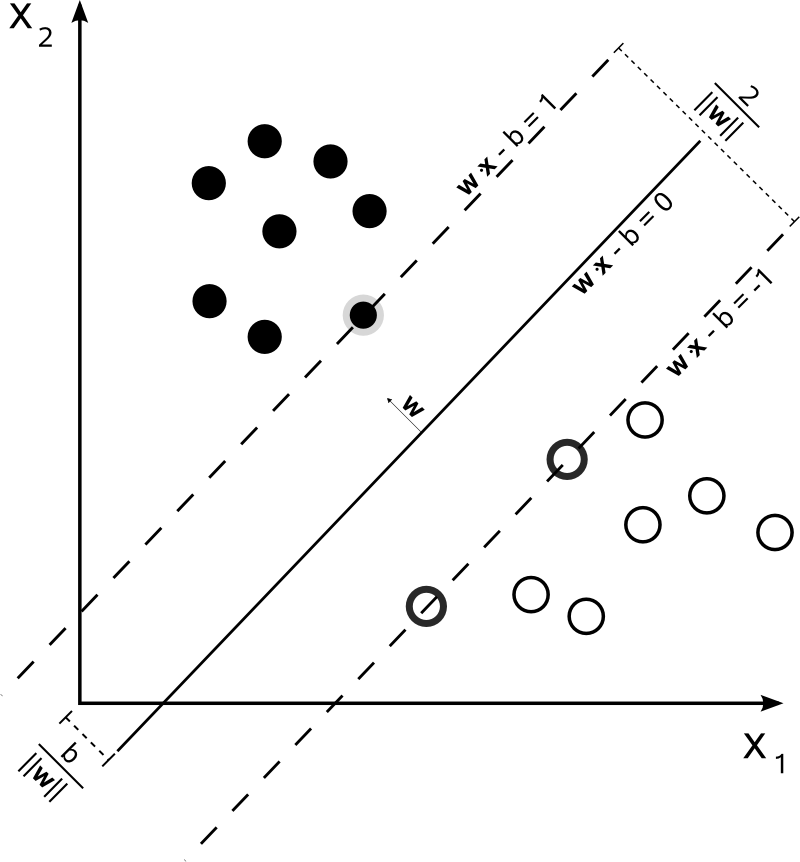
\includegraphics[width=0.7\columnwidth]{img/svm_max_margin.png}
\caption{
\label{fig:svm_max_margin}
Maximum-margin two-dimensional hyperplane and its margins for an SVM trained with samples from two classes \cite{svm_max_margin}.
}
\end{center}
\end{figure}

If we have some training data D, consisting of \textit{n} data points:

\[
	\mathcal{D} = \left\{ (\mathbf{x}_i, y_i)\mid\mathbf{x}_i \in \mathbb{R}^p,\, y_i \in \{-1,1\}\right\}_{i=1}^n
\]

we want to find a max-margin hyperplane that divides the points that have $ y_i = 1 $ from the points that have $ y_i = -1 $. The hyperplane is described by the following equation:

\begin{equation}
\label{eq:svm_hyperplane}
\mathbf{w}\cdot\mathbf{x} - b=0
\end{equation}

where $ \cdot $ is the dot product, $ \mathbf{w} $ is the normal vector to the hyperplane and $ \mathbf{x} $ represents the set of points on the hyperplane. 

For linearly separable data, there are two hyperplanes that separate the data, and the distance between them is the margin: 

\begin{align*} 
 \mathbf{w}\cdot\mathbf{x} - b &=1 \\
 \mathbf{w}\cdot\mathbf{x} - b &=-1
\end{align*}

Maximizing the margin intuitively corresponds to finding the hyperplane that is the furthest from any of the data points, as can be seen in figure \ref{fig:svm_max_margin}. Then, when we make predictions, we are less susceptible to noise and our confidence in the prediction is greater. This is because if the data point is far from the hyperplane, the probability that it lies on one side or the other of the hyperplane due to chance and not because it is of that class is much smaller. Mathematically, the distance the two hyperplanes is $ \tfrac{2}{\|\mathbf{w}\|} $, so to maximize the margin we need to minimize the $ \| \mathbf{w} \| $. 

A common method for solving this minimization problem is Platt's sequential minimization optimization (SMO) algorithm \cite{platt1998sequential}, which works by breaking the problem into the smallest possible sub-problems and then solving those analytically. 

SVM can be used to project the original data to a much higher dimensional space (in some cases even infinite-dimensional space), so that they are linearly separable in that space. The mapping to a higher dimensional space is done using a kernel function, which is used instead of the dot product in equation \eqref{eq:svm_hyperplane}.

There are several popular kernel functions that are used: 
\begin{description}
\item[Polynomial] $ k(\mathbf{x_i},\mathbf{x_j})=(\mathbf{x_i} \cdot \mathbf{x_j})^d$ \cite{goldberg2008splitsvm}
\item[Gaussian radial basis function] $ k(\mathbf{x_i},\mathbf{x_j})=\exp(-\gamma \|\mathbf{x_i} - \mathbf{x_j}\|^2)$, for $ \gamma > 0 $ \cite{Chang:2010:TTL:1756006.1859899}
\item[Hyperbolic tangent] $ k(\mathbf{x_i},\mathbf{x_j})=\tanh(\kappa \mathbf{x_i} \cdot \mathbf{x_j}+c) $, for some $ \kappa > 0 $ and $ c < 0 $ \cite{sellathurai1999separability}
\item[Wave kernel] $ k(x, y) = \frac{\theta}{\| x-y \| } \sin \frac{\| x-y \| }{\theta} $ 
\item[Power kernel] $ k(x,y) = - \lVert x-y \rVert ^d $ \cite{fleuret2003scale}
\end{description}

Kernel methods can be viewed as defining a similarity measure between two samples which is then used to classify them. \cite{Vert}

Because sometimes there is noise in the data, so it may not be possible to separate the data linearly, not even in a high dimensional space or, even if possible, this may not be desirable, because it would overfit to the data and not generalize well. In such cases, it is prefered to have a decision surfaces that makes some mistakes on the training data, but generalizes better and represents the noisy data more accurately. SVMs can be used as soft margin classifiers, allowing examples to be classified wrongly at training time, but penalizing them according to their distance to the other side of the hyperplane \cite{russell1995artificial}. In this case, the optimization problem becomes: 

\[
\arg\min_{\mathbf{w},\mathbf{\xi}, b } \left\{\frac{1}{2} \|\mathbf{w}\|^2 + C \sum_{i=1}^n \xi_i \right\}
\]

where $ \xi_i $ is non-negative slack variable and $ C $ is the penalty term. 

Because SVMs separate only two classes, when there are multiple classes to be distinguished, the ``one-vs-all'' approach can be used for classification, and is as accurate as any other approach for this problem\cite{rifkin2004defense}. In this case, one classifier is trained for each class, to distinguish it from all other classes. To make a prediction, all classifiers predict their value and the one that is used will be the one with the highest confidence score.

\subsection{Neural networks}
Neural networks are a machine learning algorithm inspired from the brain. They are modeled by neurons, that are connected to each other through synapses, which have weights. Neurons add the signals they receive from the neurons to which they are connected, pass them through an activation function, which then determines the strength of the outgoing signal of that particular neuron. 

Neural networks are usually organized into layers, each consisting of a variable number of neurons. If the connections between the neurons do not form a cycle, then this architecture is called a feedforward neural network or a \textit{multilayer perceptron} (MLP). The presence of cycles in the network gives it more representational power, at the expense of significantly more difficult training. 


\begin{figure}[h]
\begin{center}
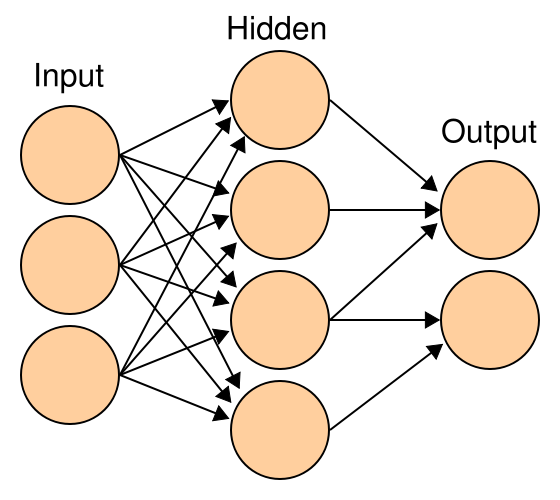
\includegraphics[width=0.7\columnwidth]{img/artificial_neural_network.png}
\caption{
\label{fig:neural_network}
Neural network with one hidden layer \cite{neural_network}
}
\end{center}
\end{figure}

Some of the more popular activation functions for neurons are:

\begin{description}
\item[Threshold] \begin{eqnarray}
  \mbox{y(x)} = \left\{ 
    \begin{array}{ll} 
      0 & \mbox{if } \mathbf{w}\cdot \mathbf{x} + b \leq 0 \\
      1 & \mbox{if } \mathbf{w}\cdot \mathbf{x} + b > 0
    \end{array}
  \right.
\end{eqnarray} \cite{rosenblatt1958perceptron}
\item[Sigmoid] $ y(x) = \frac{1}{1+\exp(-\mathbf{w} \cdot \mathbf{x} -b)} $ \cite{cybenko1989approximation}
\item[Rectified Linear Units] $ y(x) = max(0, x) $ \cite{nair2010rectified}
\end{description}

A neural network with a hidden layer has been shown by Cybenko in \cite{cybenko1989approximation} to be able to approximate any measurable function to any desired accuracy, but it doesn't offer any bounds on the number of neurons required to do so. This means that in practice the number of neurons must be determined empirically, by seeing when adding more neurons doesn't decrease the error made by the neural network. 

Training in a neural network is usually done with the backpropagation algorithm invented by Paul Werbos in \cite{werbos1974beyond}. It consists of two phases. In the first one, a training example is propagated forward through the network to see what the output would be. The second phase is to back propagate the error between the actual output of the network and the expected output (the ground truth) through all the layers. This is done by taking the difference of the two values, and multiplying it with the input activation, and substracting this amount from the weights of the neural network. This is done layer by layer. Mathematically this is written as:

\[
 \Delta w_i = \alpha (t - y) \phi' x_i 
\]

where $\alpha$ is the learning rate, t is the target output, y is the obtained output,  $ \phi $ is the activation function and $ \Delta w_i $ is the amount that must be subtracted from weight $ w_i $. 

When there are many layers in a neural network, the error gradient that is backpropagated gets smaller and smaller. The result of this is that the network learns very slowly, or in pathological cases, stops learning completely. This is called the ``vanishing gradient'' problem,  studied by Hochreiter in \cite{hochreiter1998vanishing}, and is one of the reasons because of which neural networks with many layers were not very used for a long time. 

\subsection{Deep learning}

\textit{Deep learning} is a recent development in the field of neural networks that focuses on having more layers and finding ways to avoid the vanishing gradient problem.

The deep learning revolution started in 2006 when Hinton and Teh found a learning algorithm that enabled fast learning in Deep Belief Nets (DBN) \cite{hinton2006fast}. These involved training Restricted Boltzmann Machines (RBM) in an unsupervised manner and then using them to initialize the weights of the DBNs. This initialization enabled the optimization algorithms to find a solution much faster than if they would have initialized with random weights.

\begin{figure}[h]
\begin{center}
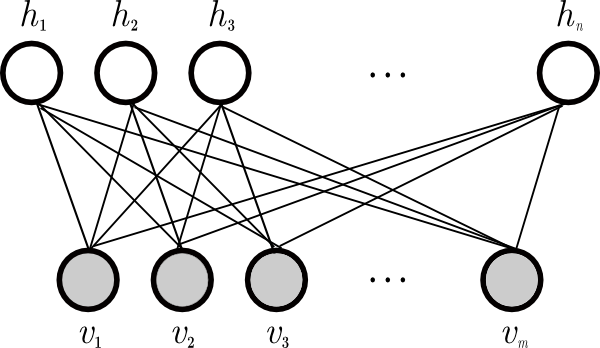
\includegraphics[width=0.7\columnwidth]{img/rbm_graph.png}
\caption{
\label{fig:rbm_graph}
RBM with m visible units and n hidden units \cite{rbm_graph}
}
\end{center}
\end{figure}

Restricted Boltzmann Machines are generative stochastic neural networks that learn a probability distribution over its inputs. Their neurons form a bipartite graph, where one layer corresponds to the input units and the other one to hidden units. The only connections that are allowed in an RBM are between a hidden unit and a visible one. This restriction is necessary to make the training of RBMs tractable. RBMs can be viewed as energy based models, which associate a scalar value to each configuration of their inputs. The desired energy function would give lower values to inputs that occur in our dataset and higher values to any other inputs. The energy function of a RBM is given by \cite{hinton2010practical}:

\[ 
	E(v,h) = -\sum_i a_i v_i - \sum_j b_j h_j -\sum_i \sum_j h_j w_{i,j} v_i	
\]

where $ a_i $ are bias weights for the visible units, $ b_j $ are the bias weights for the hidden units, $ w_{i,j} $ are the weights between the input unit $v_i$ and the hidden unit $h_j $. 

From this we can calculate the probability distributions over hidden or visible vectors in terms of the energy function:

\[
	P(v,h) = \frac{1}{Z} e^{-E(v,h)}
\]

where Z is a normalization constant (the partition function). 

Because of the restriction of RBMs to allow only connections between the two layers, they hidden units are mutually independent for a given visible unit activation, and the reverse is true as well, the visible units are mutually independent given a hidden unit activation. Mathematically this is written as:

\begin{align*}
	P(v|h) &= \prod_{i=1}^m P(v_i|h) \\
	P(h|v) &= \prod_{j=1}^n P(h_j|v) \\
	P(h_j=1|v) &= \sigma \left(b_j + \sum_{i=1}^m w_{i,j} v_i \right) \\ 
	P(v_i=1|h) &= \sigma \left(a_i + \sum_{j=1}^n w_{i,j} h_j \right)
\end{align*}

where $ \sigma $ denotes the logistic sigmoid function.

RBMs are trained using the contrastive divergence algorithm \cite{hinton2002training}. This algorithm takes a training sample $ v $, computes the activations of hidden units and samples an hidden vector $h$ from them. From $h$ construct a sample of the input units $ v'$, from which then another hidden vector $ h' $ is calculated. The difference between the outer products of $ v' $ with $ h' $ and $ v $ and $ h $ are the weight updates for the RBM. 

Another way to do unsupervised pretraining is to use autoencoders, also known as Diabolo networks \cite{bengio2009learning} . These are feedforward neural networks where the output is set to equal the input, so that they learn the identity function, but the hidden layers have certain constraints on them. The connection between the input layer and the hidden layer can be interpreted as an encoding function, while the connections between the hidden layer and the output layer can be viewed as the decoding function. These two function composed together give the identity function $ g(f(x)) = x $. 

If an autoencoder had the same number of neurons on the hidden layer as on the input layer, it would be trivial for it to learn the identity function for both the encoding and the decoding parts. This would be of no use to us. However, if there are constraints on the hidden layer, these can make the network learn useful things about the structure of the data and use it to compress or learn new, higher level features. 

The objective of the autoencoder is to minimize the reconstruction error:

\[
	L(x, y) = \|x-y\|^2
\]

The most basic type of autoencoder is the one where the constraint is that the number of neurons on the hidden layer is smaller than the number of neurons on the input layer. This prevents the network from simply memorizing the inputs, so it has to find patterns and to compress the data in order to be able to reproduce it at the output layer. 

Another type of autoencoder is a sparse autoencoder \cite{hinton2010practical}, where there is a penalty for each simultaneously activated neuron in the hidden layer. In this way, the neurons are encouraged to be activated less. Because each neuron corresponds to an extracted feature, when a neuron is activated it means that the corresponding feature is present in the input data. If the neurons have to be activated separately, then they will all learn to recognize different features. Sparsity is done by adding the following penalty term to the loss function:

\[
	\beta \sum_i ( \rho \log \frac{\rho}{\rho_j} + (1-\rho) \log \frac{1-\rho}{1-\rho_j})
\]

where $\beta $ is the term that controls the strength of the penalization, $\rho$ is the sparsity parameter, representing how often we would like a neuron to be activated. It usually has a value of $ 0.1 $. $\rho_j$ represents how often neuron \textit{j} has been activated during this training batch. 

Another way that autoencoders can learn an encoding of the input is if it corrupted with noise, but the output is still required to be the original, correct data. This is called a denoising autoencoder, introduced by Vincent Pascal in \cite{vincent2008extracting}. The noise that is added is either a gaussian noise or a binary mask that sets some of the inputs to 0. To be able to reproduce the correct output, the neural network must learn the correlations that exist between the input variables and then use them to determine when they are noisy.  

More recently, unsupervised pretraining has been abandoned in favor of better optimization methods such as the Hessian free approach introduced by Martens in \cite{martens2010deep}, new layers such as ReLU \cite{nair2010rectified}, Maxout \cite{goodfellow2013maxout}, Max-Pooling \cite{scherer2010evaluation}, better regularization with Dropout \cite{hinton2012improving}, or just by throwing more computational power at the problem, as done by Cireșan in \cite{Cire_an_2010}. In this paper, Cireșan et al. have showed that using a GPU to train the neural network using the same layers that have existed for 20 years, can obtain results on the MNIST dataset which were the state-of-the-art at the time, using only dataset augmentations. 

The Hessian free optimization method involves taking into account 2nd order information about the gradient in order to avoid pathological cases in the surface of the loss function. While classic optimization algorithms often waste a lot of time bouncing in valleys, the Hessian free speeds up the process of going through the valley. It improves upon other second order optimization methods such as Newton's method, because they require the computation of the Hessian matrix, which can be difficult to calculate analytically and for n parameters requires $ \mathcal{O}(n^2) $ storage space and time steps, which is unfeasible in practice for neural networks with millions of parameters. The Hessian free method sidesteps the need to calculate this expensive Hessian matrix, replacing it with applying Conjugate Gradient on the second order Taylor expansion of the function to optimize. 

ReLU units have the activation function $ y(x) = max(0,x) $. This is an approximation to an infinite sum of binary gaussian units, all with a different offset. The advantage of using ReLU is that it is very quick to compute, it doesn't have a vanishing gradient problem because on the $ (0, +\infty) $ area it's derivative is always 1. A disadvantage is that ReLU units don't saturate, meaning that they don't have an upper limit on the value they can take. 

Dropout is a regularization technique that is specific to neural networks. It works by applying a binary mask to a layer in a MLP during training, selecting which inputs to be active and which to turn off. This mask is changed randomly for each example or batch of examples. The effect of this is that each neuron has to learn to make decisions individually, without relying on getting ``help'' from other neurons, thus preventing their co-adaptation. Dropout can also be viewed mathematically as a way of doing model averaging over all the models that contain only a subset of the input variables. Normally, training a model for all the subsets would be computationally expensive, the number of subsets growing exponentially, but in this way, by training one model we can achieve the same effect. 

Maxout layers were designed to work together with dropout, and they are simply feed-forward layers that have the activation function $ y_i(x) = max_{j\in[1,k]} z_{ij} $, where $ z_{ij} = x^T W_{...ij} +b_{ij} $ and $ W \in \mathbb{R}^{d \times m \times k } $ and $ b \in \mathbb{R} ^{ m \times k } $ are learned parameters. What this does is take the maximum over \textit{k} features. This can then be interpreted as constructing piecewise linear approximations to any arbitrary convex functions. In this way, maxout networks learn not just the way hidden units are connected, but also what are the best activation functions to use. 

Convolutional neural networks have also gained popularity in deep learning. While having been used before, in the problem of handwritten zip code recognition \cite{lecun1989backpropagation} or face recognition \cite{lawrence1997face}, with recent advances in computing power they have become feasible to use and have been applied with great success in computer vision and speech recognition. They are inspired by the way the visual cortex works. A convolutional layer, instead of having connections between all the input neurons and all the output ones, is sparsely connected. Each neuron in a convolutional layer is connected only to the closest neurons to him spatially. In addition to this, the weights between the neurons are shared, being replicated over all neurons. This means that any interesting features will be detected regardless of their position in the input image, because the weights are the same. Convolutional layers are usually alternated with sub-sampling layers, that pick only the best or strongest response from the previous layer. An example of such an architecture is LeNet, which can be seen in figure \ref{fig:lenet_conv}. 


\begin{figure}[h]
\begin{center}
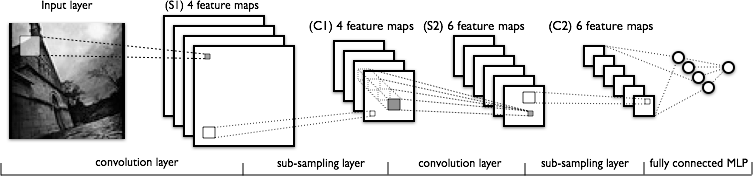
\includegraphics[width=0.7\columnwidth]{img/mylenet.png}
\caption{
\label{fig:lenet_conv}
Architecure of neural networks from the LeNet family \cite{lenet_conv}
}
\end{center}
\end{figure}